Desde la concepción de Kwii Platform los usuarios son el atractivo y objetivo de la aplicación, por lo tanto ofrecemos una plataforma la cual permita gran fluidez durante su uso aun cuando hay muchos Kwiers haciendo uso de la aplicación. En está sección se hará una descripción detallada de las tacticas usadas por la plataforma para poder sostener estas condiciones.

\subsection{Escalabilidad}

Como se detalla en la sección \ref{sub:cyc}, la aplicación cuenta con diferentes componentes que se encargan de tareas especificas para el funcionamiento de la aplicación, haciendo uso de la técnica de replicación logramos que tareas críticas como el envío de mensajes sea repartido entre diferentes instancias de los componentes.

\noindent Como se logra ver en la figura \ref{fig:stressTest}, aplicando la replicación se logra un mejor desempeño y una mayor capacidad de respuesta que de haber una sola instancia de los componentes, esta mejora en el rendimiento se logra haciendo un uso correcto de balanceadores de carga, los cuales distribuyen las peticiones provenientes de los clientes de manera equitativa entre las diferentes instancias de los componentes,y de esta manera se minimiza el estrés recibido por cada componente por separado.

\begin{figure}[h]
    \centering
    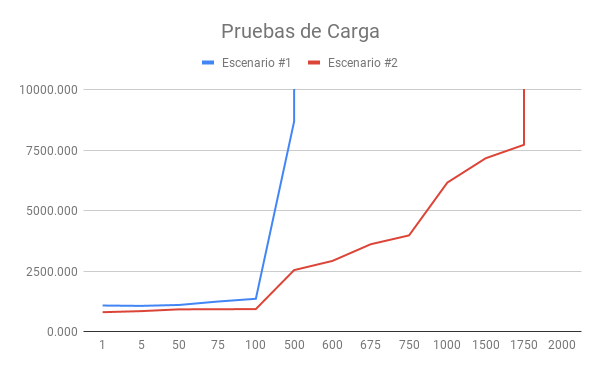
\includegraphics[width=9cm]{Figures/P5/stressTest.png}
    \caption{Escenario \#1: Componentes sin replicar, Escenario \#2 Componentes replicados}
    \label{fig:stressTest}
\end{figure}

\subsection{Resiliencia}

Además de los micro-servicios, también se realizo una replicación de los componentes de Base de Datos, lo cual permite que en caso de algún imprevisto la aplicación pueda mantener y recuperar los datos de manera automática. 
Esta replicación se hizo para las siguientes bases de datos:
\begin{itemize}
    \item Chats\\
    Siendo la base de datos fundamental para la funcionalidad core de Kwii Platform se hace una replicación en un esquema maestro-esclavo en donde la instancia maestro es la encargada de responder peticiones, además se sincroniza con la instancia esclavo de manera que en caso de un fallo de la primera esta pueda relevar las funciones manteniendo la integridad de los datos.
    \item Usuarios\\
    Para mantener a salvo y actualizada la información de los usuarios se hace una replicación de esta base en un esquema maestro-maestro en donde ambos componentes tienen autorizado tanto lectura como escritura de manera tal que cualquiera puede responder las peticiones de la aplicación.
\end{itemize}

\subsection{Alta Disponibilidad}

Como medida adicional Kwii Platform cuenta con sus componentes distribuidos en los siguientes puntos geográficos:
\begin{itemize}
    \item Estados Unidos:
    \begin{itemize}
        \item Iowa
        \item Oregon
        \item Los Angeles
        \item Virginia
    \end{itemize}
    \item Montreal - Canadá
    \item São Paulo - Brasil
\end{itemize}

\noindent Esta distribucion nos asegura que la aplicación se encuentre disponible para su uso aun en circunstancias extremas que involucren la infraestructura física de la misma.